\title{Service-Based Architecture}
\author{Richard Thomas}
\date{\week{4}}

\maketitle

\section{Introduction}

Service-based architecture is one of the simpler, but still flexible, distributed architectural styles.
It provides good support for delivering quality attributes of modularity, availability, deployability, and simplicity (in the context of a distributed system).
The key characteristic of a service-based architecture is that it uses domain partitioning, and each domain becomes its own distributed service.
This partitioning provides high-level modularisation that helps ensure the domain partitions are independent of each other.
The distribution of domains means that multiple instances of a service can be made available through a load balancer,
providing better availability and some level of scalability.

Many medium-sized bespoke systems\footnote{\emph{Bespoke systems} are custom designed and built for a single organisation.}
are built using a service-based architecture.
For example, an on-line store might be partitioned into services such as ProductBrowsing,
ProductPurchasing, ProductFulfilment, InventoryManagement, and CustomerAccountManagement.
Each of these could be independent distributed services that use a shared database.

\vspace{2mm}
\begin{definition}[Service-based Architecture]
    The system is partitioned into business domains that are deployed as distributed services.\\
    Functionality is delivered through a user interface that interacts with the domain services.
\end{definition}

\begin{figure}[h!]
    \begin{adjustwidth}{-7.5mm}{-7.5mm}
        \centering
        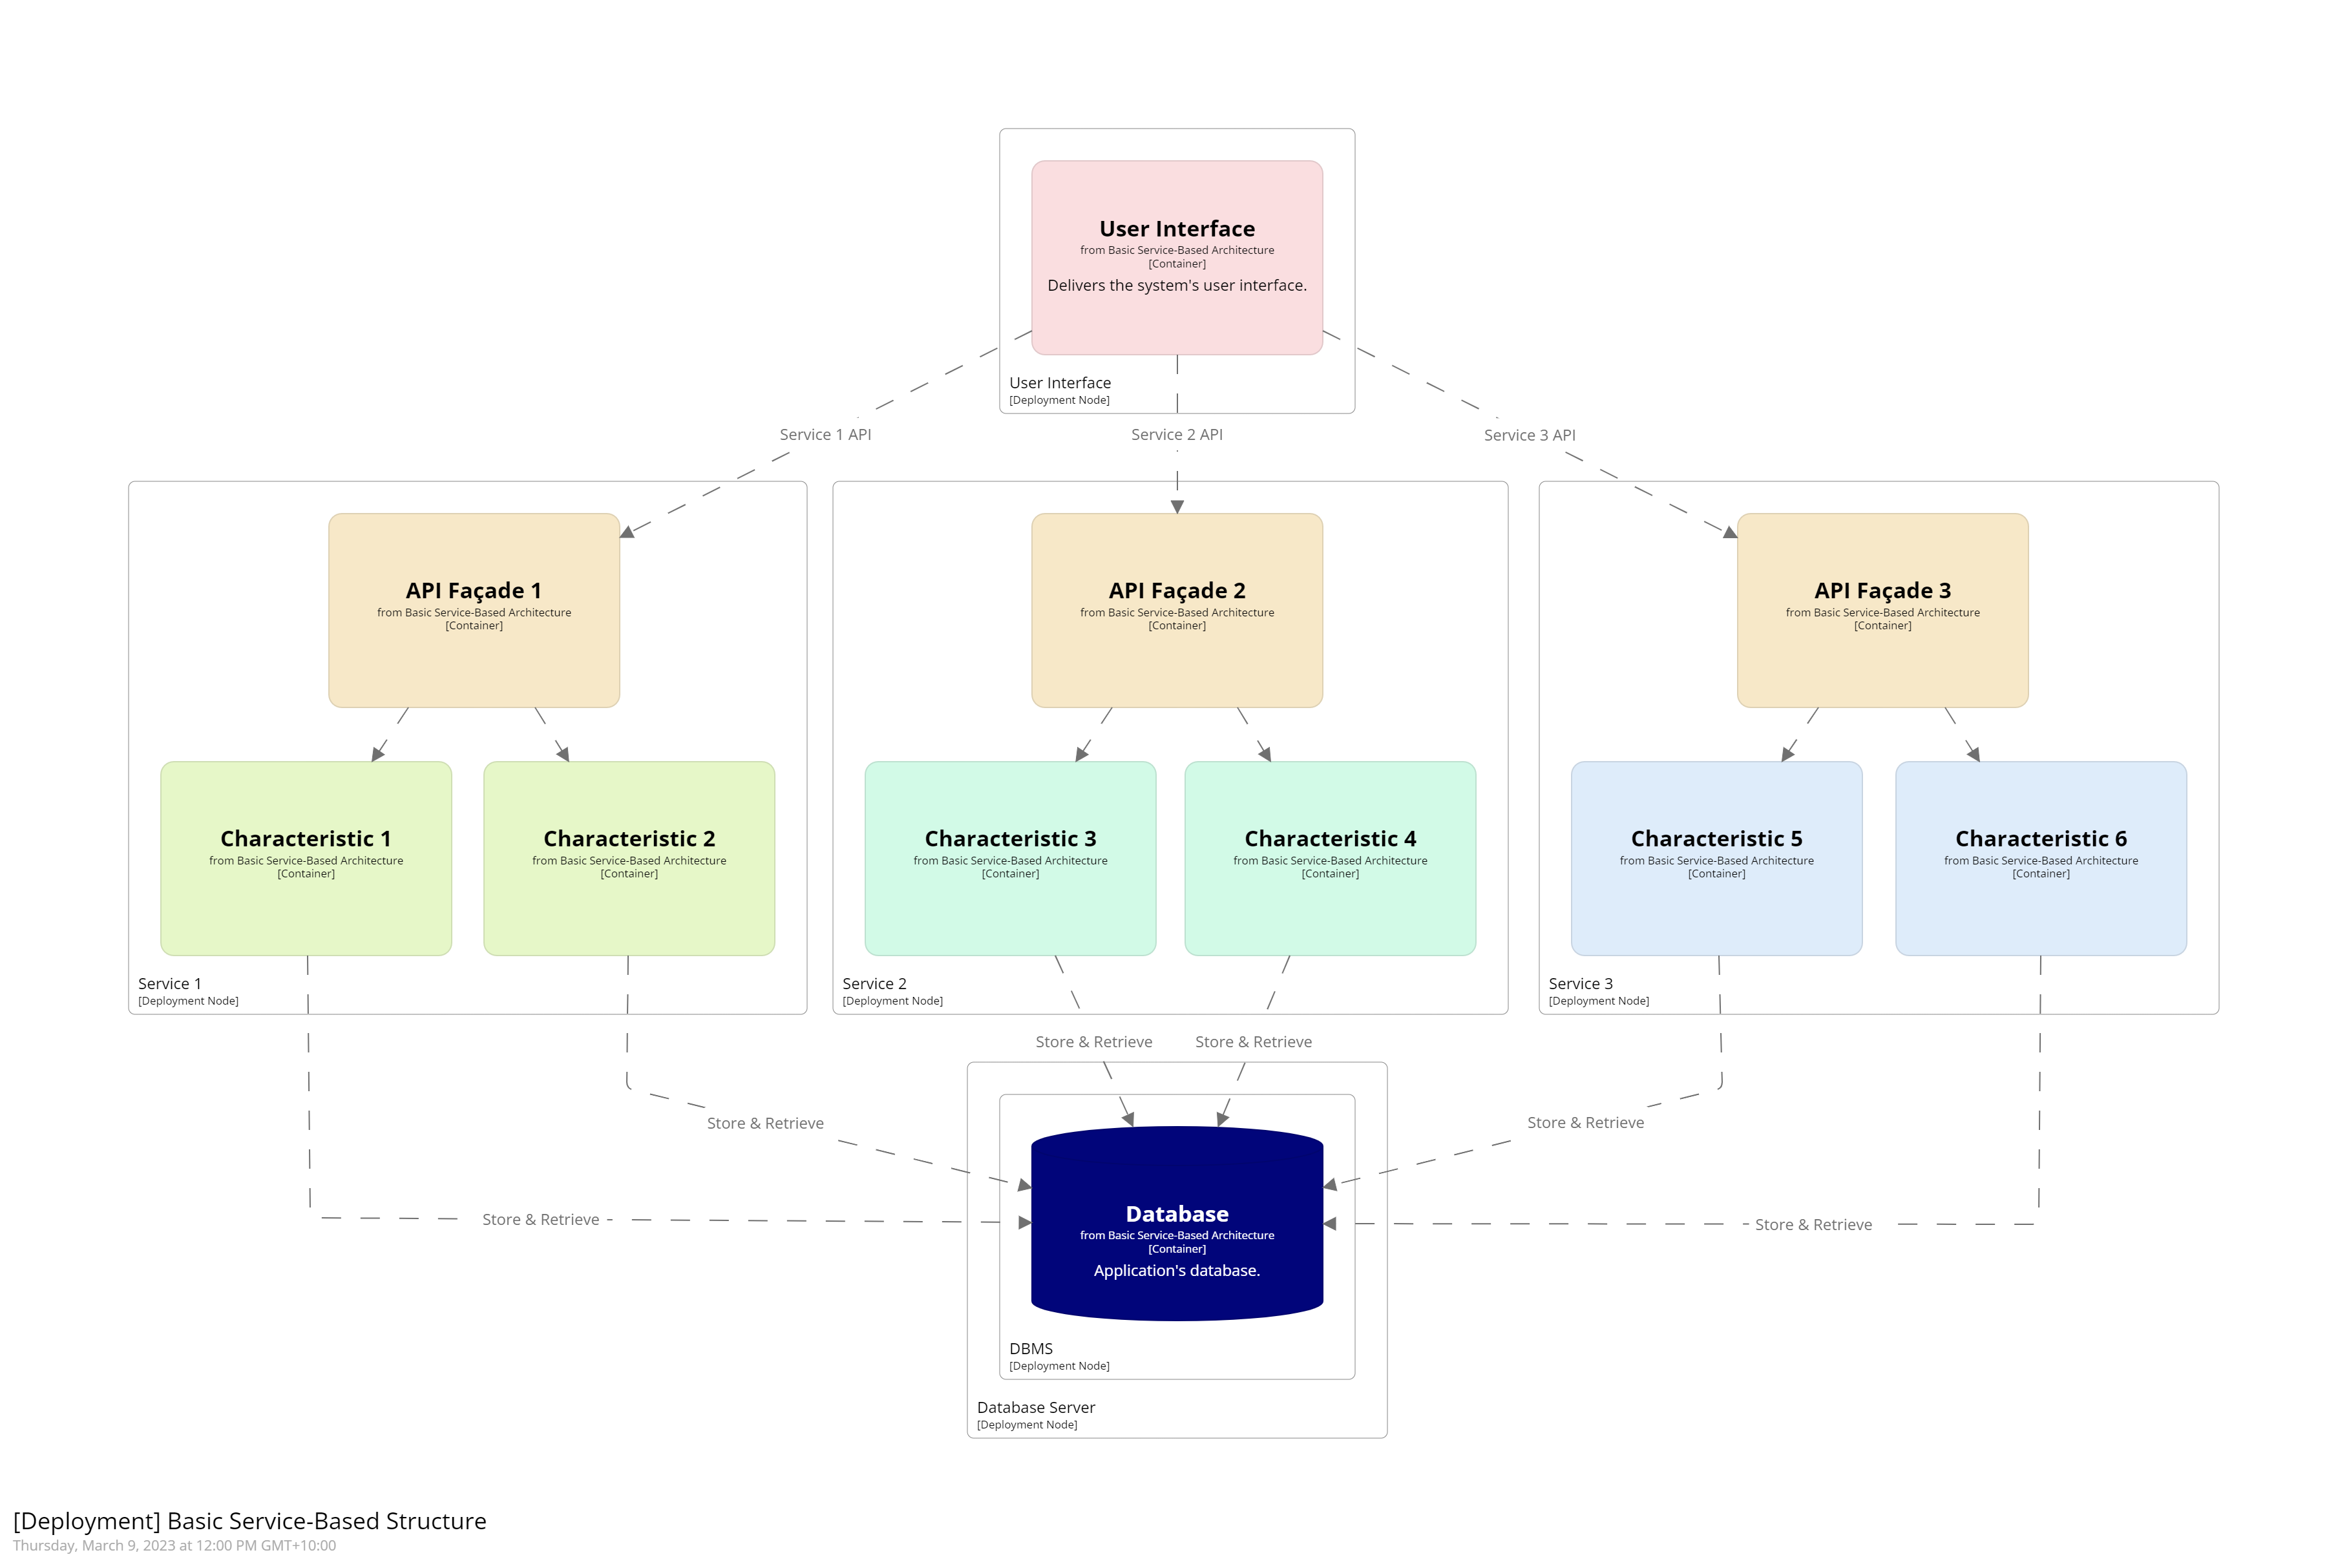
\includegraphics[trim=39 43 19 44,clip,width=0.95\paperwidth]{diagrams/general-service-based-arch.png}
    \end{adjustwidth}
    \caption{Service-based architecture -- general structure.}
    \label{fig:service-based-arch}
\end{figure}


\section{Terminology}

The service-based architecture consists of four elements.
The \emph{user interface}, \emph{services}, \emph{service APIs}, and \emph{database}, as shown in figure \ref{fig:service-based-arch}.

\begin{description}
    \item[User Interface] provides users access to the system functionality.
    \item[Services] implement functionality for a single, independent business process.
    \item[Service APIs] provide a communication mechanism between the user interface and each service.
    \item[Database] stores the persistent data for the system.
\end{description}

The user interface runs as a standalone process to manage user interactions.
It communicates with the services through their service APIs to invoke system behaviour.
This requires a remote access communication protocol, such as REST, a message transport service,
remote method invocation, \link{SOAP}{https://www.w3schools.com/xml/xml_soap.asp} or some other protocol.

To reduce coupling between the user interface and the service APIs, and to provide easier extensibility, the user interface often uses a
\link{service locator design pattern}{https://www.baeldung.com/java-service-locator-pattern} to manage access to the services%
\footnote{Martin Fowler provides good commentary about using the service locator pattern at \url{https://martinfowler.com/articles/injection.html\#UsingAServiceLocator}.
He expands further on some tradeoffs of the pattern than other more superficial descriptions of the pattern.}.
This provides a registry of the services and the details of the API of each service.
The user interface uses the registry to retrieve an object that communicates with a service through its API.
This also makes it easier to add new services to the application, as the details of the new service are encapsulated in the registry.

Services implement the application logic for independent business processes.
These are often called ``coarse-grained'' services, as each one implements a significant part of the system's functionality.
Each service is deployed on its own computing infrastructure.
Commonly, there is a single instance of each service but it is possible to run multiple instances of services.
Multiple instances of services improves availability because if one instance goes down, other instances can handle future requests from the user interface.
To provide higher reliability, in the context of running multiple instances of a service, it should implement the
\link{stateless service pattern}{https://www.oreilly.com/library/view/design-patterns-and/9781786463593/f47b37fc-6fc9-4f0b-8cd9-2f41cb364509.xhtml}.
A system running multiple instances of a service, that does not implement the stateless service pattern,
would still have higher availability if a service instance went down, as other instances could handle future requests.
But, any user in the middle of performing a business process would need to restart their activity, thus lowering system reliability.

Services implement their own service API using the \link{façade design pattern}{https://refactoring.guru/design-patterns/facade}.
This defines the communication protocol used between the user interface and the service.
For simplicity, usually all services use the same communication protocol.
The façade design pattern reduces coupling between the user interface and the services,
as the user interface does not depend on the implementation details of the services.

The service API provides the benefit that different user interfaces can all use the same services.
For example, an application with web and mobile interfaces could use the same set of distributed domain services.

The database stores persistent data for the system.
Often, a single database is shared by all the services as it is common that some data will be shared between services.
A shared database makes it easier to maintain data integrity and consistency.
This is because each service implements a single business process
and can usually perform all transaction management related to the data involved in the process.
For example, the ProductPurchasing service for an on-line store can manage the entire database transaction for making an order.
If the product is no longer available or payment fails, the service can rollback the transaction to ensure data integrity.


\section{Design Considerations}\label{sec:design-considerations}

A service-based architecture is typically used for medium-sized systems.
This is because the user interface interacts with all services through their APIs.
The user interface becomes more complicated when it has to deal with many services.
If the services follow the common approach of using a shared database,
it means the the greater the number of services, the more complicated the database design becomes.
There is also a potential performance bottleneck if many services are using a shared database.
Strategies to improve database performance, like replicated databases, defeat some of the benefits of a shared database (e.g. consistency).
Typically a service-based architecture will have six to twelve domain services.
There is no specific upper or lower limit on the number of services allowed,
it is a tradeoff that architects make based on all the requirements for the system.

Coarsed-grained services will usually have some internal complexity that requires some architectural structure.
This internal structure may follow either technical or domain partitioning.
Technical partitioning will typically consist of three layers, the API façade, business logic and persistence.
Domain partitioning will break the service domain into smaller components related to each part of the domain's behaviour.
For example, the ProductPurchasing service domain may have components for the internal behaviours of checking out,
payment and inventory adjustment. Payment would use an API to process payment through a financial service gateway.
Figure \ref{fig:service-partitions} provides an example of the structure for both technical and domain partitioning of a service.

\begin{figure}[h!]
    \centering
    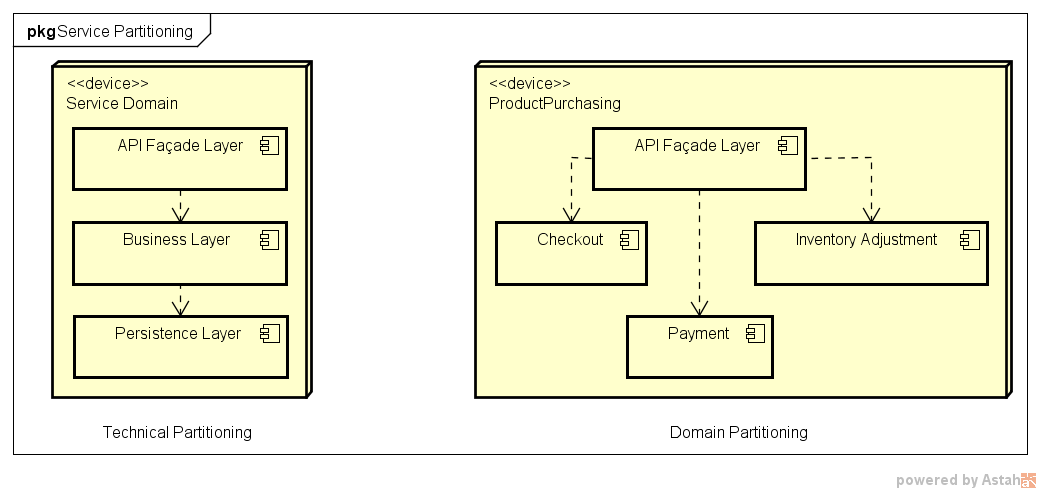
\includegraphics[trim=38 38 19 45,clip,width=\textwidth]{diagrams/service-partitions.png}
    \vspace{-10pt}
    \caption{Partitioning options for a service domain.}
    \label{fig:service-partitions}
\end{figure}

Consequences of a shared database are increased data coupling between the services and lower testability.
Increased data coupling means that if one service changes its persistent data,
then all services that share that data need to be updated, as well as the tables storing the data in the database.
Lower testability is the consequence of shared data and services implementing complete business processes.
A small change to one part of the service requires the entire service to be tested,
and all other services that share data with the service also need to be tested.

To mitigate data coupling, design a minimal set of shared (or \emph{common}) persistent objects and their corresponding tables in the database.
Implement a library containing the shared persistent classes that is used by all services.
Restrict changes to the shared persistent classes and their database tables.
Changes may only occur after consideration of the consequences to all services.
A variation is to not only have shared persistent objects,
but other persistent objects that are only shared with a subset of services.

Each service may have its own set of persistent objects and corresponding database tables.
These are independent of other services, so there are no external consequences to changing these within a service.
Figure \ref{fig:db-logical-partitioning} is an example of shared persistent objects and a service with its own persistent objects.

\begin{figure}[h!]
    \centering
    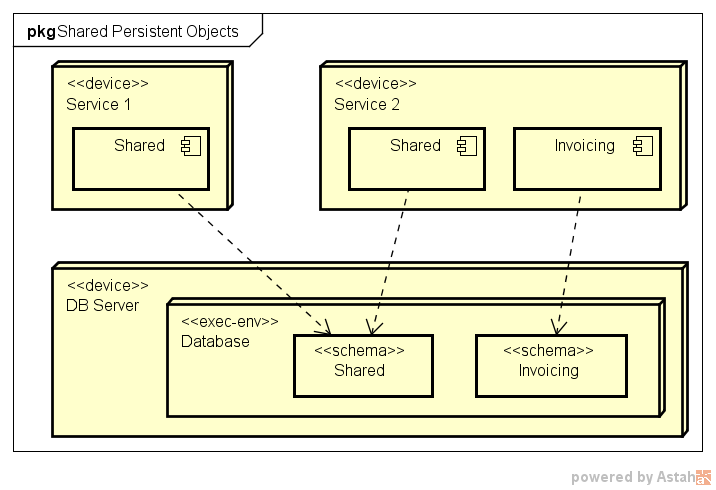
\includegraphics[trim=37 37 20 44,clip,width=0.61\textwidth]{diagrams/db-logical-partitioning.png}
    \caption{Database logical partitioning example.}
    \label{fig:db-logical-partitioning}
\end{figure}

\section{Service-Based Principles}
There are a couple of principles which should be maintained when designing a service-based architecture
to produce a simple, maintainable, deployable and modular designs.

\vspace{1mm}
\begin{definition}[Independent Service Principle]\label{independent-service}
    Services should be independent, with no dependencies on other services.
\end{definition}

Services should be independent of each other.
If a service depends on other services they either cannot be deployed separately,
or they require communication protocols between services, which increases the coupling and complexity of the system design.

\vspace{1mm}
\begin{definition}[API Abstraction Principle]\label{api-abstraction}
    Services should provide an API that hides implementation details.
\end{definition}

The user interface should not depend on implementation details of any services.
Each service should publish an API that is a layer of abstraction between the service's implementation and the rest of the system.
This provides an interface through which the service can be used and reduces coupling between the service and its users.
In a service-based architecture, the user interface is the primary client of service APIs but it is not necessarily the only client.
Auditing services may also need to use domain services.
In more sophisticated environments, services may be shared across different systems.


\section{Extensions}

There are a few common variations of the service-based architecture to consider.

\subsection{Separate Databases}

The first variation  we will consider is to have separate databases for each service.
This extends the idea of logical partitioning your database, as described in section \ref{sec:design-considerations}.
Figure \ref{fig:separate-dbs} shows a few options of how this can be implemented.

\begin{figure}[h!]
    \begin{adjustwidth}{-5mm}{-5mm}
        \centering
        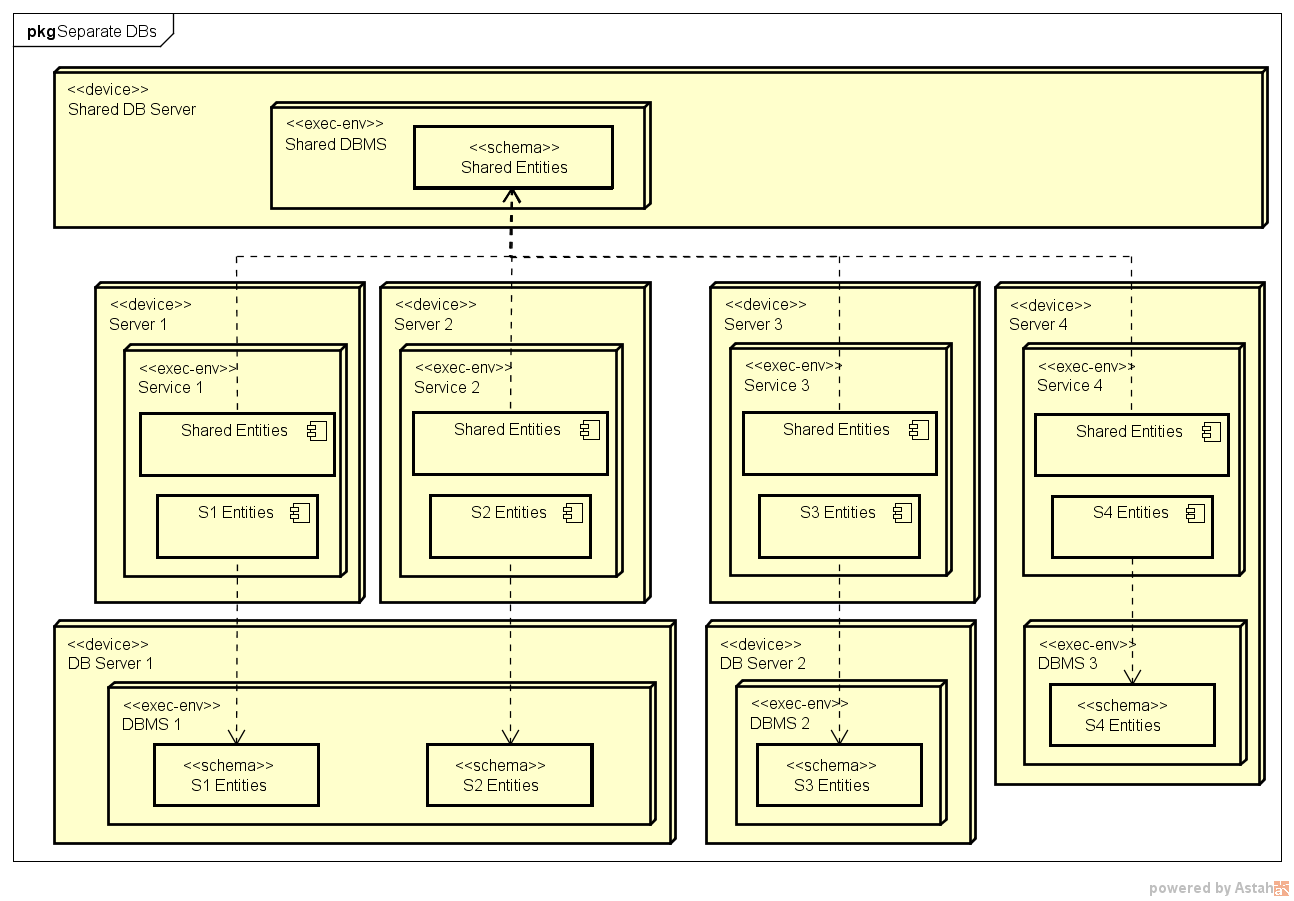
\includegraphics[trim=39 42 18 48,clip,width=0.92\paperwidth]{diagrams/separate-dbs.png}
    \end{adjustwidth}
    \caption{Separate databases example.}
    \label{fig:separate-dbs}
\end{figure}

In figure \ref{fig:separate-dbs}, there is a shared database that contains the entity data that is shared across services.
Service 1 and 2 are deployed on separate servers but share a single database server that hosts different tables for each service.
Service 3 has communicates with its own database server that hosts its tables.
Service 4 uses a database that is running on the same server as the service.

Each of these approaches have their own advantages and disadvantages.
A key consideration is whether a service has enough unique data to make it worth creating a separate database for just the service.
If most data is shared between services, it may be easier to implement the system with just a single shared database.
If there is some data that is unique to some services, a single database server
with either logical partitioning of the data or even independent database services,
may provide enough performance for the system.
A separate database server for some or all services provides greater flexibility for scaling,
if database performance is likely to become a bottleneck for the service.
Running an independent database on the same server as the service provides easier communication with the database
and may suit cases where an independent database is useful but it is not large enough to warrant to run on its own server.

\subsection{Separate User Interfaces}

A similar variation can be applied to the user interface, so that there are separate user interfaces for some services.
This allows separate interfaces to be implemented for different user interface domains
(e.g. standard users, power users, administrators, ...).
Figure \ref{fig:separate-uis} shows some options of how this can be implemented.

\begin{figure}[h!]
    \centering
    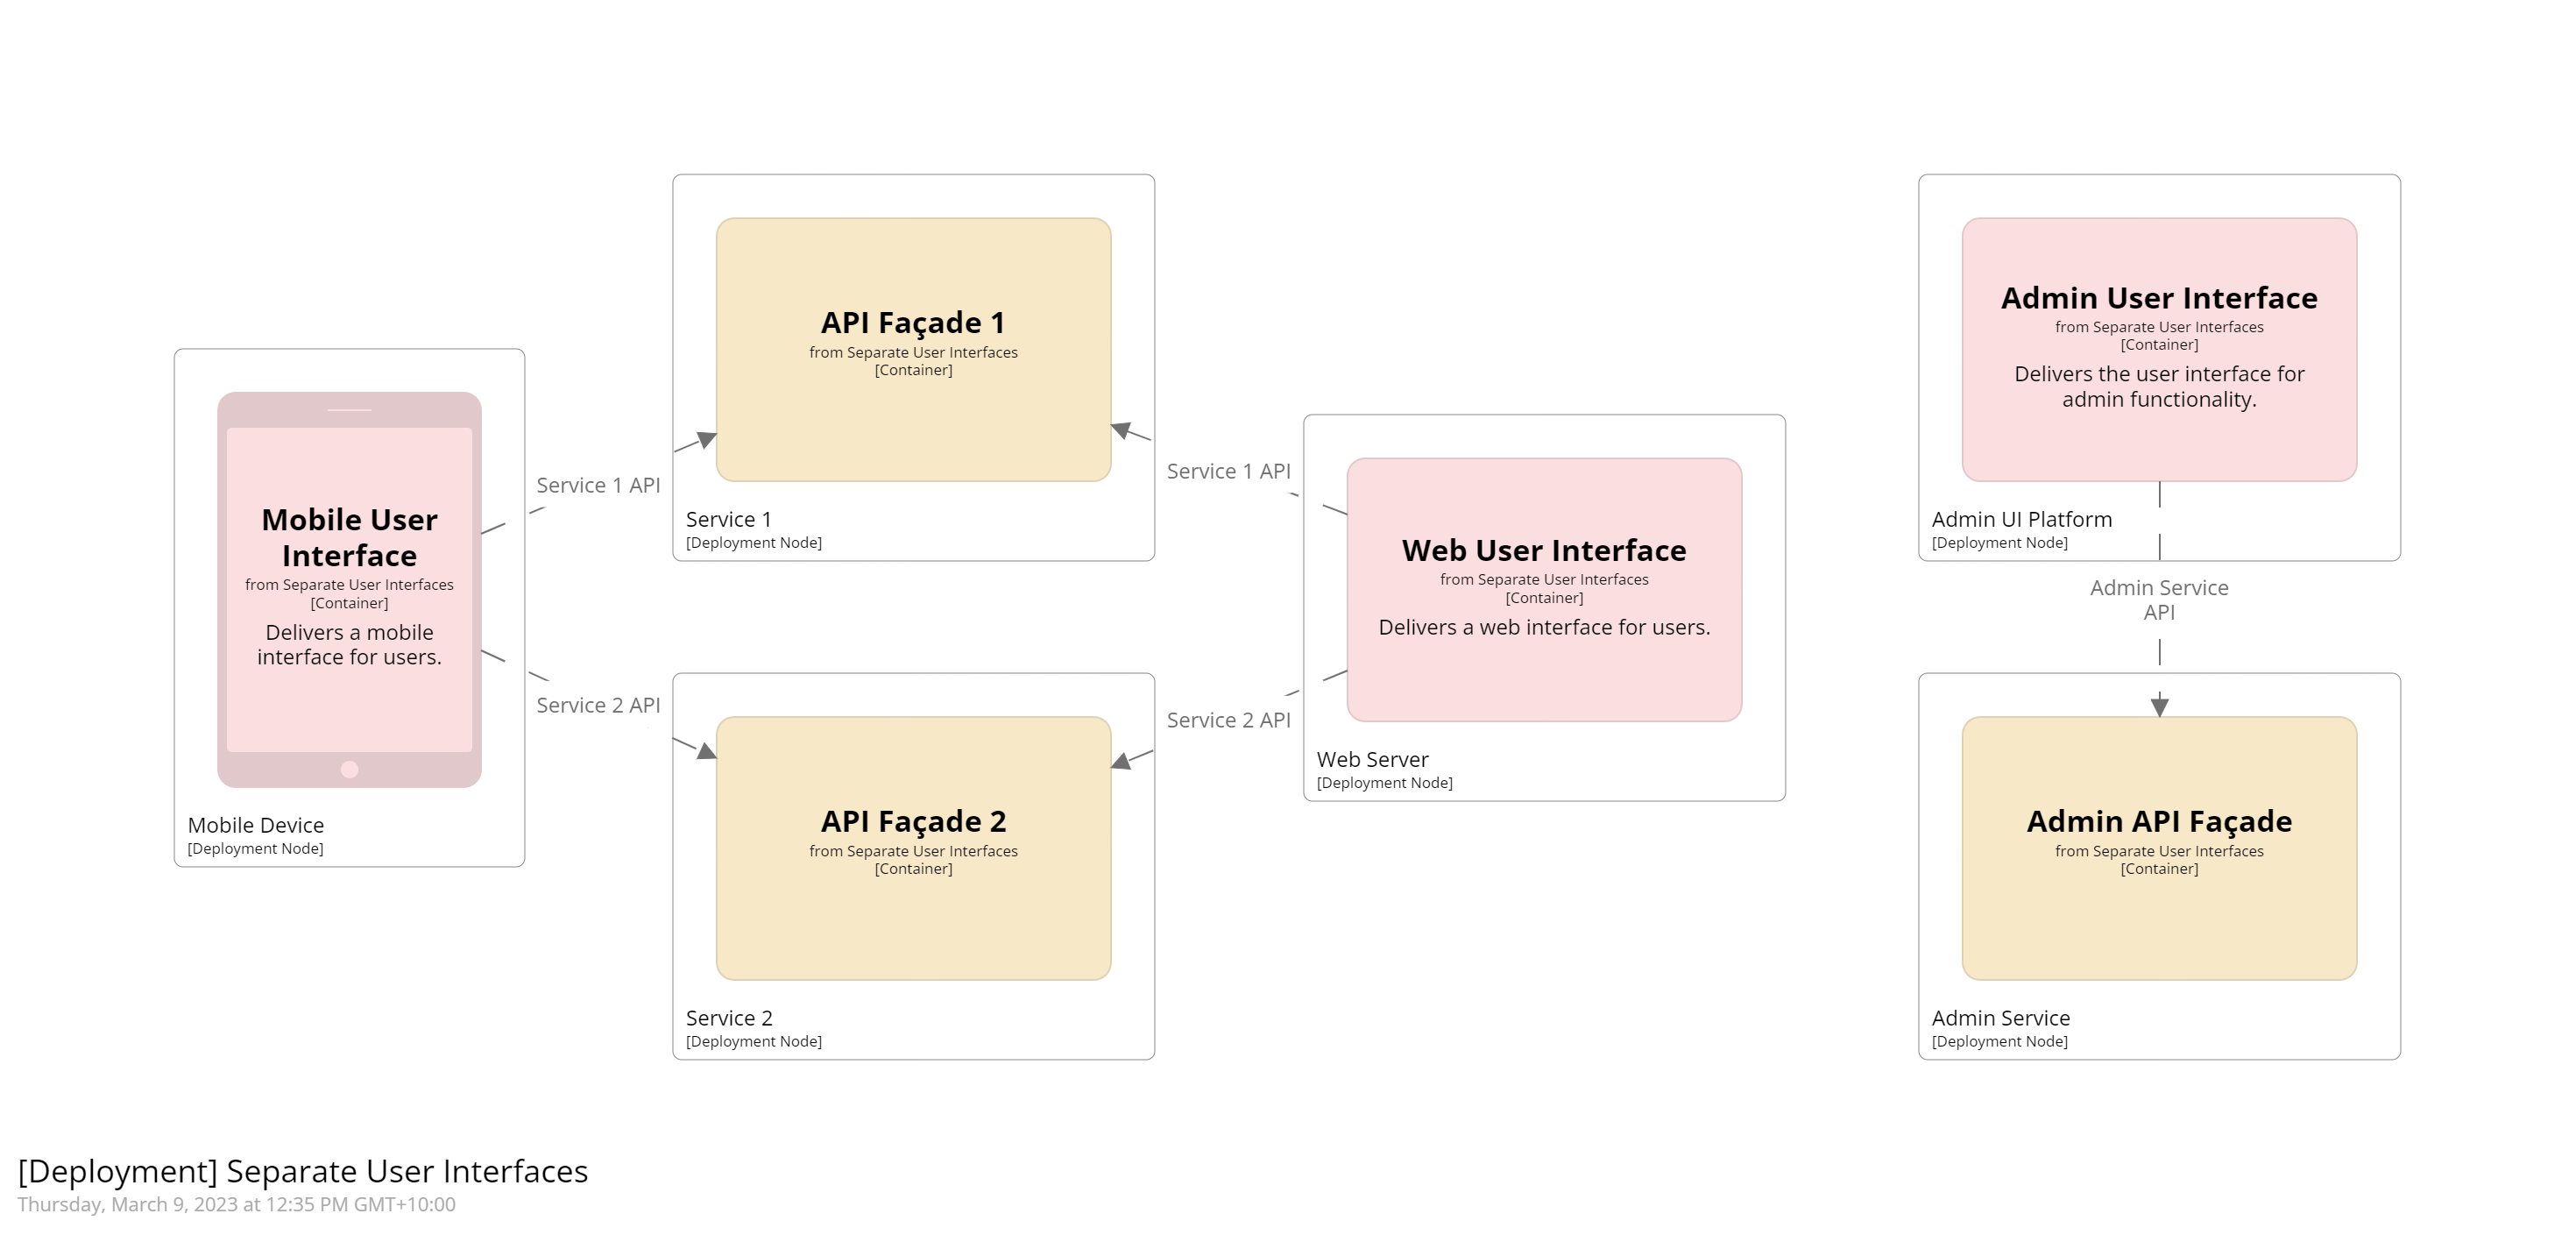
\includegraphics[trim=40 42 19 45,clip,width=0.9\textwidth]{diagrams/separate-uis.png}
    \caption{Separate user interfaces example.}
    \label{fig:separate-uis}
\end{figure}

In figure \ref{fig:separate-uis}, there is one user interface that interacts with two services,
like the single interface in the general structure shown in figure \ref{fig:service-based-arch}.
There are then two interfaces that interact with service 3.
A benefit of the service API is that it allows multiple interfaces to be implemented to work with the backend services.

\subsection{API Layer}

It is possible to place an API layer between the user interface and the services,
as shown in figure \ref{fig:api-layer}.
The API layer is a reverse proxy or gateway that provides access to the services,
while hiding details of the services.

\begin{figure}[h!]
    \centering
    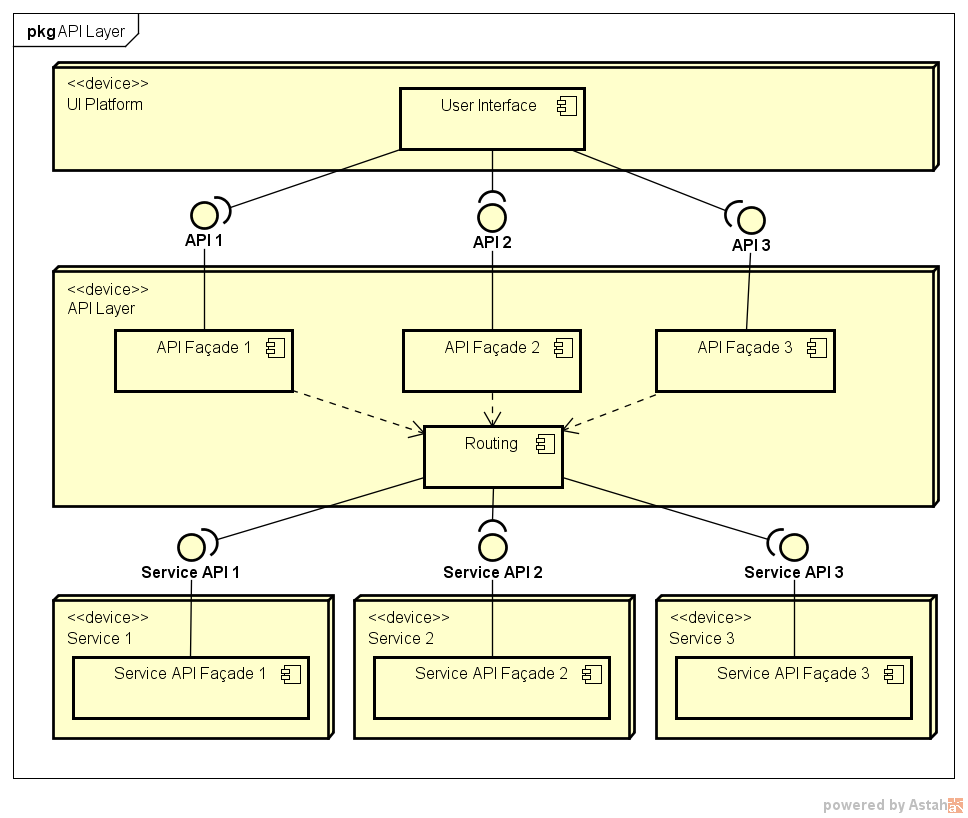
\includegraphics[trim=39 37 21 42,clip,width=0.85\textwidth]{diagrams/api-layer.png}
    \caption{API layer separating the user interface from services.}
    \label{fig:api-layer}
\end{figure}

If any domain services are used by external systems, a reverse proxy hides the internal network structure of your system's architecture.
This extra layer of abstraction means that you can expose a different interface to external systems than to internal systems.
This can help deliver the security principle of least privilege.

The API layer allows the implementation of \emph{cross-cutting} concerns to be separated from the user interface.
For example security policies, user access logging, or service discovery could be implemented in the API layer.

Service discovery allows new services to be registered and provides a mechanism for clients to ``discover'' the new services.
The API layer would provide an interface that allows services to be registered, including information about their interface.
The API layer would also provide an interface to clients that allows them to query what services are available
and to retrieve an interface that the client can use to access the service through the API layer.

The API layer can also perform load balancing by delegating service requests to different servers running the same domain service.


\section{Service Oriented Architecture}

Service Oriented Architecture (SOA) is an extension of service-based architecture.
In SOA, each service implements a single business process and provides one or more interfaces that allow access to its functionality.
The primary purpose of the API layer is to provide a robust service discovery platform and to implement security policies.
Systems are implemented by integrating a set of services to deliver the required functionality.
Consequently, the user interface is part of the system being implemented and not part of the service architecture.
SOA requires each service to be independent of the others, including very low data coupling.
Typically in SOA, each service would have its own database.

SOA sounds like a good idea, but in practice many organisations made compromises that neutered much of the expected benefits.
Business processes are often not perfectly independent and there is often data dependencies between processes.
If these dependencies are not managed well, the services are not independent.
This results in services having to be used together, which reduces their reusability and composability.

Another common issue was a poor service discovery implementation.
One problem was that the mechanism to discover new services required too much knowledge about the services.
This results in the clients needing to know the services, before they can discover them.
Another problem was poor interface design, that caused dependencies on some implementation details of the services.

Microservices were designed to deliver the promised benefits of SOA without some of the implementation issues.
In particular, microservices deliver much smaller elements of functionality, reducing the possibility of tight coupling between services.
There are challenges in designing and delivering microservices to achieve the benefits.
These will be explored later in the course.


\section{Conclusion}

Service-based architecture is an approach to designing a distributed system that is not too complex.
Domain services provide natural modularity and deployability characteristics in the architecture design.
Well designed service APIs improve the encapsulation and hide implementation details of the services.
